\section{More DP}
\begin{frame}{}
  \begin{center}
    {\bf Part I -- More DP}
  \end{center}
\end{frame}

\subsection{Cutting Sticks}
\begin{frame}
  \frametitle{Choosing the right DP table size -- "Cutting Sticks"}

  {\smaller
    \begin{block}{Problem Description}
      \begin{itemize}
      \item In a stick of length $l$ ($1 \leq l \leq 1000$)
      \item Make $N$ cuts at positions $\text{cuts} = \{c_1, c_2,
        \ldots, c_N\}$ $(1 \leq N \leq 50)$
      \item The cost of a cut is the size of the sub-stick that you cut.
      \item What order of cuts \structure{minimize the cost}?
      \end{itemize}
  \end{block}

  \medskip

  \structure{Example:} $l=100, N=3, \text{cuts}=\{25,50,75\}$

  \begin{center}
    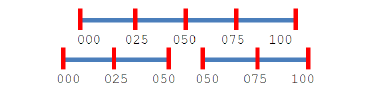
\includegraphics[width=0.6\textwidth]{../img/cuttingsticks}
  \end{center}

  \begin{itemize}
  \item Sequence 1: 25, 50, 75. Cost: 100 + 75 + 50 = 225
  \item Sequence 2: 50, 25, 75. Cost: 100 + 50 + 50 = 200
  \end{itemize}
  }
\end{frame}

\begin{frame}
  \frametitle{Cutting Sticks -- Thinking about the Problem}

  {\smaller
    \begin{center}
      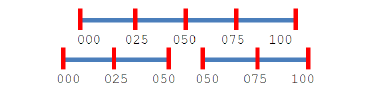
\includegraphics[width=0.55\textwidth]{../img/cuttingsticks}
      \begin{itemize}
      \item Sequence 1: 25, 50, 75. Cost: 100 + 75 + 50 = 225
      \item Sequence 2: 50, 25, 75. Cost: 100 + 50 + 50 = 200
      \end{itemize}
    \end{center}

    \begin{exampleblock}{Part 1 -- consider full search}
      \begin{itemize}
      \item What is the algorithm for a full search?
      \item What is the complexity of this algorithm? And the maximum time?
      \end{itemize}
    \end{exampleblock}

    \begin{exampleblock}{Part 2 -- Consider DP}
      \begin{itemize}
      \item This problems smells of {\bf DP}. (Find Maximum, several choices)
      \item Think about the states (DP table) and how to change between them (transition)
      \end{itemize}
    \end{exampleblock}

  }
\end{frame}

\begin{frame}
  \frametitle{utting Sticks -- Top Down DP (Recursive Function)}
  {\smaller
    \begin{center}
      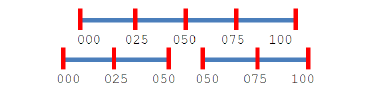
\includegraphics[width=0.6\textwidth]{../img/cuttingsticks}
      \begin{itemize}
      \item Sequence 1: 25, 50, 75. Cost: 100 + 75 + 50 = 225
      \item Sequence 2: 50, 25, 75. Cost: 100 + 50 + 50 = 200
      \end{itemize}
    \end{center}

    \begin{block}{Recurrence}
      Let's think of a \structure{Top-down DP} based on a recursive function:
      \begin{itemize}
      \item $A = \{0, c_1, c_2, \ldots c_N, N+2\}$ is the set of all cutting
        points, plus the start and end point.
      \item $\text{cost}(a_i,a_j) = \text{dist}(a_i,a_j) + \text{min}_{i\leq k\leq j}
        (\text{cost}(a_i,a_k) + \text{cost}(a_k,a_j))$
      \item $\text{cost}(a_i,a_i) = 0$
      \end{itemize}
      This requires at most a $(N,N)$ DP table for memoization, and O(N) for each iteration.
    \end{block}

  }
\end{frame}

\subsection{ACORN}
\begin{frame}
  \frametitle{DP Problem 2 -- Acorn}

  \begin{columns}
    \column{0.4\textwidth}
    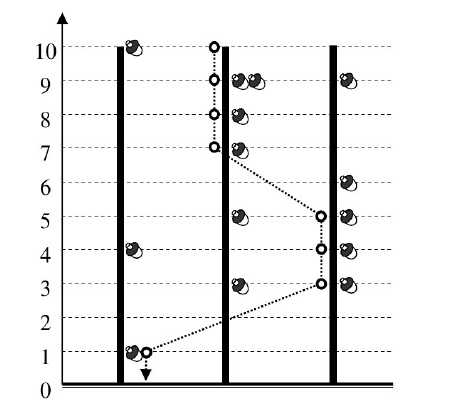
\includegraphics[width=1\textwidth]{img/acorn}
    \column{0.6\textwidth}
    \ppagenote{Acorn Image from CPBook4 (Steven Halim)}

    \begin{itemize}
    \item Begin at the top of a tree, and get the maximum number of acorns.
    \item You can go down {\bf 1 height} on the tree.
    \item OR {\bf change tree} for the cost of {\bf f height}\\
      (In this figure, $f = 2$)

      \bigskip

    \item Number of trees: $ 1 \leq T \leq 2000$
    \item Height of trees: $ 1 \leq H \leq 2000$
    \item Length of fall : $ 1 \leq f \leq 500$
    \end{itemize}
  \end{columns}

  \begin{block}{}
    \begin{itemize}
      \item First, it is worth to think about the full search size;
      \item But this problem smells of DP -- can you think of a {\bf transition} and a {\bf state table}?
    \end{itemize}
  \end{block}
\end{frame}

\begin{frame}
  \frametitle{ACORN -- Simple Recurrence}
  \begin{columns}[T]
    \column{0.3\textwidth}
    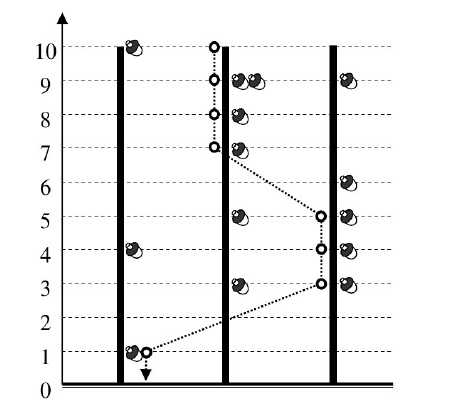
\includegraphics[width=1\textwidth]{img/acorn}
    \column{0.7\textwidth}
    \begin{block}{Simple Recurrence}
      \begin{itemize}
      \item acorn$[t_i][h]$ -- number of acorns in tree {\bf $t_i$} at height {\bf $h$}
        \bigskip

      \item cost$(t_i,0)$ = acorn$[t_i][0]$
        \bigskip

      \item cost$(t_i,j)$ = acorn$[t_i][j]$ + \\
        \hspace{1.6cm}max$_{k\neq t_i}($cost$(t_i,j-1)$, cost$(t_k,j-f))$\\
        (Don't forget to check $j-f < 0$)
        \bigskip

      \item Final cost: max$_{1\leq i \leq T}($cost$[t_i][H])$
      \end{itemize}
    \end{block}
  \end{columns}

  \vfill

  \begin{center}
    \alert{QUIZ:} What is the problem with this recurrence?
  \end{center}
\end{frame}

\begin{frame}
  \frametitle{ACORN -- Finding a Better DP table}

    \begin{alertblock}{}
      The DP table of last slide is A[H][T], with size $2000*2000=4M$.
      Each function call is $O(H*T*T)$, so total complexity is
      $4M*2000=8B$
    \end{alertblock}

    \medskip

    \begin{itemize}
    \item Cost of changing tree is constant for any two trees.
    \item It is not necessary to keep all trees, only the best.
    \end{itemize}

    \medskip

    \begin{block}{Better Recurrence -- $O(H*T)$}
      We use the table dp$[H]$ which contains the best solution at height H.

      \medskip

      \begin{itemize}
      \item $\text{dp}[0] = \text{max}_{1\leq j\leq T}\text{acorn}[j][0]$
       \medskip

      \item $\text{acorn}[j][i] += \text{max}(\text{acorn}[j][i-1], \text{max}[i-f])$
        \medskip

      \item $\text{dp}[i] = \text{max}_{1\leq j\leq T}(\text{acorn}[j][i])$
      \end{itemize}
    \end{block}
\end{frame}
